\documentclass[12pt]{article}
%Gummi|065|=)
\usepackage{amsmath, amsfonts, amssymb}
\usepackage[landscape, margin=0.5in]{geometry}
\usepackage{xcolor}
\usepackage{graphicx}
\newcommand{\off}[1]{}
\DeclareMathSizes{20}{30}{21}{18}

\usepackage{tikz}

\title{\textbf{ Domino Tilings }}
\author{John D Mangual}
\date{}
\begin{document}

\fontfamily{qag}\selectfont \fontsize{25}{30}\selectfont

\maketitle

% note AVOID THE WORDS 'Ratner Theorem' instead explain what it is

\noindent It is time to review that classic problem, domino tilings\footnote{There are possibly two tracks we can do.  A coding track and a theory track.  In this iteration of review we will focus on \textbf{theory} with a mimimum of coding.   Certain steps, which for that community are quite clear, I'll take a lot more work to understand.  So I will expend a lot of effort re-writing existing arguments in a way that hopefully makes sense to everybody .  
In my defense, my teacher was David Speyer -- who is an expert in domino tilings -- and even he wasn't aware of certain things I was telling him.  Indeed, we will take many detours that look somewhat frivolous or purely for my own curiosity... because the lecture notes are for me.}.  

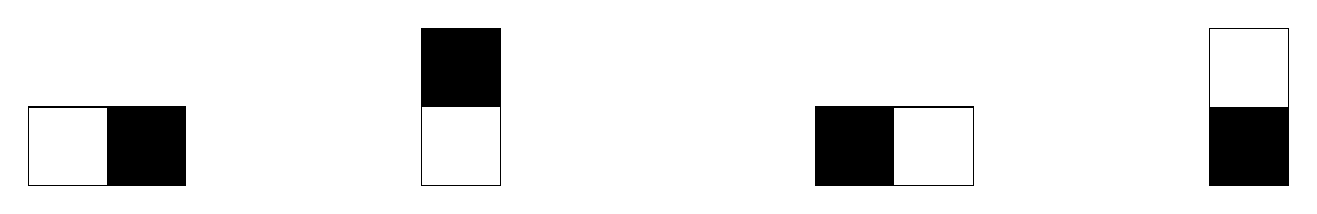
\begin{tikzpicture}

\draw (0,0)--(2,0)--(2,1)--(0,1)--cycle;
\path[fill=black] (1,0)--(2,0)--(2,1)--(1,1)--cycle;

\begin{scope}[xshift=5cm]
\draw (0,0)--(1,0)--(1,2)--(0,2)--cycle;
\path[fill=black] (0,1)--(1,1)--(1,2)--(0,2)--cycle;
\end{scope}

\begin{scope}[xshift=10cm]
\draw (0,0)--(2,0)--(2,1)--(0,1)--cycle;
\path[fill=black] (0,0)--(1,0)--(1,1)--(0,1)--cycle;
\end{scope}

\begin{scope}[xshift=15cm]
\draw (0,0)--(1,0)--(1,2)--(0,2)--cycle;
\path[fill=black] (0,0)--(1,0)--(1,1)--(0,1)--cycle;
\end{scope}

\end{tikzpicture}
\newline \noindent I liked Solomon Golomb's book on Polyominoes.  We can do  a bit if we focus on just one type of piece such as an L or a T.
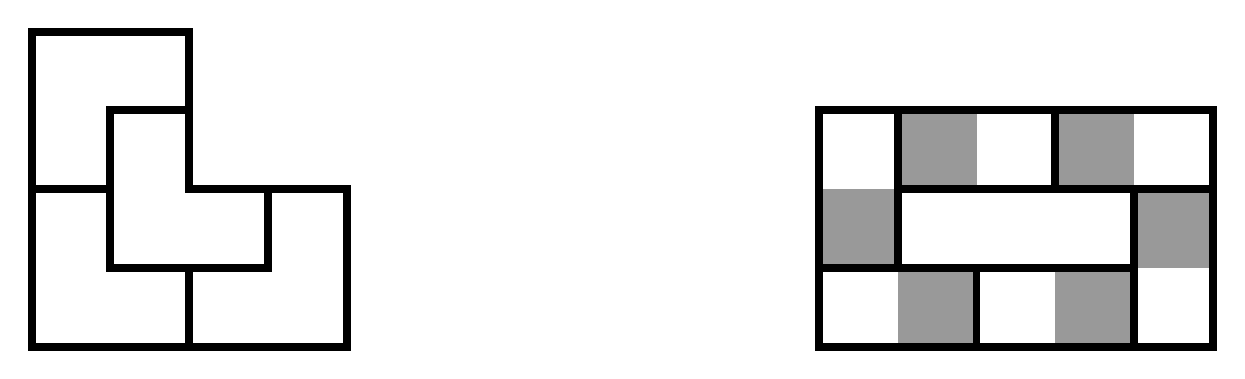
\begin{tikzpicture}

\draw[line width=0.1cm] (0,0)--(2,0)--(2,1)--(1,1)--(1,2)--(0,2)--cycle;

\draw[line width=0.1cm] (2,0)--(4,0)--(4,2)--(3,2)--(3,1)--(2,1)--cycle;

\draw[line width=0.1cm] (1,1)--(3,1)--(3,2)--(2,2)--(2,3)--(1,3)--cycle;

\draw[line width=0.1cm] (0,2)--(1,2)--(1,3)--(2,3)--(2,4)--(0,4)--cycle;

\begin{scope}[xshift=10cm]


\path[fill=black!40!white] (1,0)--(2,0)--(2,1)--(1,1)--cycle;
\draw[line width=0.1cm] (0,0)--(2,0)--(2,1)--(0,1)--cycle;

\path[fill=black!40!white] (3,0)--(4,0)--(4,1)--(3,1)--cycle;
\draw[line width=0.1cm] (2,0)--(4,0)--(4,1)--(2,1)--cycle;

\path[fill=black!40!white] (5,1)--(5,2)--(4,2)--(4,1)--cycle;
\draw[line width=0.1cm] (4,0)--(5,0)--(5,2)--(4,2)--cycle;

\path[fill=black!40!white] (3,2)--(4,2)--(4,3)--(3,3)--cycle;
\draw[line width=0.1cm] (3,2)--(5,2)--(5,3)--(3,3)--cycle;

\path[fill=black!40!white] (1,2)--(2,2)--(2,3)--(1,3)--cycle;
\draw[line width=0.1cm] (1,2)--(3,2)--(3,3)--(1,3)--cycle;

\path[fill=black!40!white] (0,1)--(1,1)--(1,2)--(0,2)--cycle;
\draw[line width=0.1cm] (0,1)--(1,1)--(1,3)--(0,3)--cycle;

\end{scope}

\end{tikzpicture}

\newpage

\noindent \textbf{Q1:} Why is Checkerboard Tiling Correct\footnote{Figure should be an $8 \times 8$ checkboard with two corners removed.  Can you tile with $2 \times 1$ rectangles?  Depending on your choice of corners, answer is \textbf{YES} or \textbf{NO}.}?

\newpage

\noindent \textbf{Q2:} Is that Really a Circle in the Middle?

\includegraphics{"30x30 Aztec Diamond"}

\newpage


\fontfamily{qag}\selectfont \fontsize{12}{10}\selectfont

\begin{thebibliography}{}

\item William Thurston \textbf{Conway's Tiling Groups} \texttt{ http://www.jstor.org/stable/2324578}

\item William Jockusch,James Propp, Peter Shor \textbf{Random Domino Tilings and the Arctic Circle Theorem} \texttt{arXiv:math/9801068}


\item Alexei Borodin, Leonid Petrov \newline
 \textbf{Integrable probability: From representation theory to Macdonald processes} \hspace{4em}\;
\texttt{ arXiv:1310.8007}  \newline
\textbf{Lectures on Integrable probability: Stochastic vertex models and symmetric functions}\texttt{  arXiv:1605.01349}

\item Alexei Borodin, Vadim Gorin \textbf{Lectures on integrable probability} \texttt{arXiv:1212.3351}

\item Kurt Johansson.  \textbf{Discrete orthogonal polynomial ensembles and the Plancherel measure} \texttt{arXiv:math/9906120}

\item Michael Freedman, Matthew Headrick \textbf{Bit threads and holographic entanglement} \texttt{ arXiv:1604.00354}
\end{thebibliography}


\end{document}

